\documentclass[a4paper,12pt]{article}
\usepackage[utf8]{inputenc}
\usepackage{url}
\usepackage{graphicx}
\setlength{\parindent}{0.0cm}


\begin{document}
\title{TiRa labra - Testausdokumentti} 
\author{Jarmo Isotalo}
\maketitle

\section{Testausdokumentti}

\subsection{Mitä on testattu?}
Testit testaavat irrallisesti oleellisimmat (d-)keon metodit. Lisäksi testaavat kekojen järjestykseen liittyviä ominaisuuksia. Eli testit lisäävät kekoon N kpl Satunnaisia arvoja väliltä 0-1000 ja poistavat ne sen jälkeen. Testit tarkistavat että arvot tulevat suuruusjärjestyksessä.\\

Testit on toteutettu rspec-ohjelmalla ajettaviksi.

\subsection{Testien ajaminen}
Testit voidaan suorittaa kansiossa  \emph{heap/Heap/} suorittamalla komennon \emph{rspec spec/}. Tämä ajaa kaikki testit ja raportoi mahdollisista virheistä komentorivi käyttöliittymäänsä.
Testien ajaminen päivittää joka kerralla koodin testien kattavuuden laskennan. 

Testien kattavuuden näkee tiedostosta: 
\emph{heaps/Heap/src/doc/index.html} 


\subsection{Benchmark}
Kekojen toimintaa voi benchmarkata suorittamalla \emph{heaps/Heap/benchmark/} kansiossa olevan \emph{my\_benchmark\_spec.rb}  tiedoston.

Esimerkiksi kansiossa \emph{heaps/Heap/} ollessa komentorivillä \emph{rspec benchmark/}

Tämä tulostaa seuraavanlaisen kaavion:
Kaaviosta puuttu ääkköset ohjelmien yhteensopivuuden parantamiseksi.
\newpage
\scriptsize
\begin{verbatim}

                            user     system      total        real
Binaarikeko 100:lla     0.000000   0.000000   0.000000 (  0.004949)
Kolmikeko 100:lla       0.000000   0.000000   0.000000 (  0.003697)
D-keko 10 100:lla       0.010000   0.000000   0.010000 (  0.003469)
Binaarikeko 30000:lla   3.800000   0.010000   3.810000 (  3.825025)
Kolmikeko 30000:lla     2.840000   0.010000   2.850000 (  2.870184)
D-keko 10 30000:lla     3.140000   0.010000   3.150000 (  3.169556)
DHeap 1 5000:lla        0.580000   0.000000   0.580000 (  0.617604)
DHeap 2 5000:lla        0.420000   0.000000   0.420000 (  0.425953)
DHeap 3 5000:lla        0.390000   0.010000   0.400000 (  0.391032)
DHeap 4 5000:lla        0.400000   0.000000   0.400000 (  0.406708)
DHeap 5 5000:lla        0.470000   0.000000   0.470000 (  0.472169)
DHeap 6 5000:lla        0.490000   0.000000   0.490000 (  0.514938)
DHeap 7 5000:lla        0.380000   0.000000   0.380000 (  0.380401)
DHeap 8 5000:lla        0.370000   0.000000   0.370000 (  0.370969)
DHeap 9 5000:lla        0.420000   0.000000   0.420000 (  0.420706)
DHeap 10 5000:lla       0.390000   0.000000   0.390000 (  0.392438)
DHeap 11 5000:lla       0.390000   0.000000   0.390000 (  0.402889)
DHeap 12 5000:lla       0.370000   0.010000   0.380000 (  0.367923)
DHeap 13 5000:lla       0.370000   0.000000   0.370000 (  0.372817)
DHeap 14 5000:lla       0.400000   0.000000   0.400000 (  0.399144)
DHeap 15 5000:lla       0.370000   0.000000   0.370000 (  0.374943)
DHeap 16 5000:lla       0.390000   0.000000   0.390000 (  0.395118)
DHeap 17 5000:lla       0.400000   0.000000   0.400000 (  0.401337)
DHeap 18 5000:lla       0.400000   0.000000   0.400000 (  0.396923)
DHeap 19 5000:lla       0.400000   0.000000   0.400000 (  0.405545)
DHeap 20 5000:lla       0.390000   0.000000   0.390000 (  0.392820)
DHeap 21 5000:lla       0.390000   0.000000   0.390000 (  0.391228)
DHeap 22 5000:lla       0.420000   0.010000   0.430000 (  0.420219)
DHeap 23 5000:lla       0.370000   0.000000   0.370000 (  0.377934)
DHeap 24 5000:lla       0.400000   0.000000   0.400000 (  0.397912)
DHeap 25 5000:lla       0.380000   0.000000   0.380000 (  0.388313)
DHeap 26 5000:lla       0.410000   0.000000   0.410000 (  0.409097)
DHeap 27 5000:lla       0.380000   0.000000   0.380000 (  0.381889)
DHeap 28 5000:lla       0.400000   0.000000   0.400000 (  0.401615)
DHeap 29 5000:lla       0.410000   0.000000   0.410000 (  0.415548)
DHeap 30 5000:lla       0.410000   0.000000   0.410000 (  0.416339)
DHeap 31 5000:lla       0.410000   0.010000   0.420000 (  0.412884)
DHeap 32 5000:lla       0.390000   0.000000   0.390000 (  0.391757)
DHeap 33 5000:lla       0.380000   0.000000   0.380000 (  0.380364)
DHeap 34 5000:lla       0.370000   0.000000   0.370000 (  0.375173)
DHeap 35 5000:lla       0.390000   0.000000   0.390000 (  0.385576)
DHeap 36 5000:lla       0.390000   0.000000   0.390000 (  0.395305)
DHeap 37 5000:lla       0.370000   0.000000   0.370000 (  0.374957)
DHeap 38 5000:lla       0.430000   0.000000   0.430000 (  0.432587)
DHeap 39 5000:lla       0.410000   0.000000   0.410000 (  0.420339)
DHeap 40 5000:lla       0.390000   0.010000   0.400000 (  0.386936)
DHeap 41 5000:lla       0.400000   0.000000   0.400000 (  0.409444)
DHeap 42 5000:lla       0.380000   0.000000   0.380000 (  0.382405)
DHeap 43 5000:lla       0.400000   0.000000   0.400000 (  0.395761)
DHeap 44 5000:lla       0.400000   0.000000   0.400000 (  0.404396)
DHeap 45 5000:lla       0.380000   0.000000   0.380000 (  0.387226)
DHeap 46 5000:lla       0.420000   0.000000   0.420000 (  0.425065)
DHeap 47 5000:lla       0.380000   0.000000   0.380000 (  0.375571)
DHeap 48 5000:lla       0.380000   0.000000   0.380000 (  0.388668)
DHeap 49 5000:lla       0.420000   0.010000   0.430000 (  0.425790)
DHeap 50 5000:lla       0.380000   0.000000   0.380000 (  0.379787)
\end{verbatim} 
\normalsize
Alun testissä  D-keon D oli 10. Alla on testattu D-keon D koon vaikutus operaatioiden nopeuteen. Alimmissa benchmarkeissa on lisätty 5000 satunnasta kokonaislukua D-kekoon.

Testit on ajettu i7 mac book prolla.\\
Tässä vielä kuvaaja yllä olevista ajoista.\\
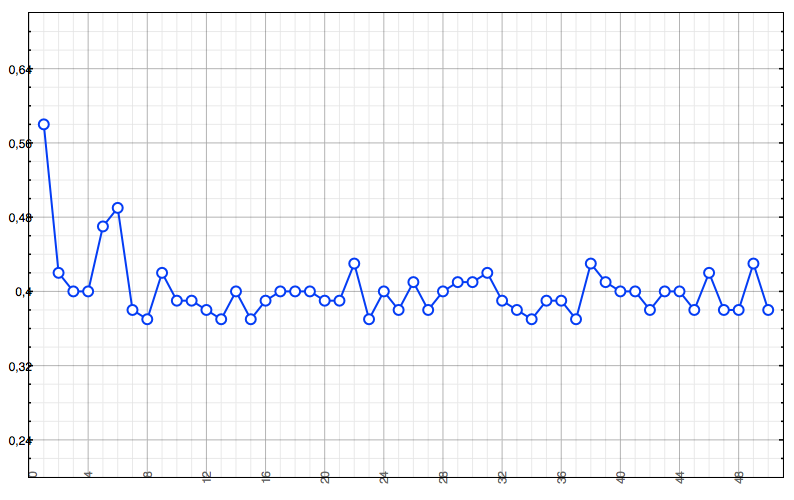
\includegraphics[scale=0.55]{graph.png}
\newpage
Vastaavat testit suoritettuna jrubyllä.

\scriptsize
\begin{verbatim}

                            user     system      total        real
Binaarikeko 100:lla     0.004000   0.000000   0.004000 (  0.004000)
Kolmikeko 100:lla       0.002000   0.000000   0.002000 (  0.002000)
D-keko 10 100:lla       0.002000   0.000000   0.002000 (  0.002000)
Binaarikeko 30000:lla   1.490000   0.000000   1.490000 (  1.490000)
Kolmikeko 30000:lla     1.100000   0.000000   1.100000 (  1.100000)
D-keko 10 30000:lla     1.262000   0.000000   1.262000 (  1.262000)
DHeap 1 5000:lla        0.157000   0.000000   0.157000 (  0.157000)
DHeap 2 5000:lla        0.155000   0.000000   0.155000 (  0.155000)
DHeap 3 5000:lla        0.156000   0.000000   0.156000 (  0.156000)
DHeap 4 5000:lla        0.176000   0.000000   0.176000 (  0.176000)
DHeap 5 5000:lla        0.173000   0.000000   0.173000 (  0.173000)
DHeap 6 5000:lla        0.153000   0.000000   0.153000 (  0.153000)
DHeap 7 5000:lla        0.186000   0.000000   0.186000 (  0.186000)
DHeap 8 5000:lla        0.166000   0.000000   0.166000 (  0.166000)
DHeap 9 5000:lla        0.156000   0.000000   0.156000 (  0.156000)
DHeap 10 5000:lla       0.155000   0.000000   0.155000 (  0.155000)
DHeap 11 5000:lla       0.153000   0.000000   0.153000 (  0.153000)
DHeap 12 5000:lla       0.154000   0.000000   0.154000 (  0.154000)
DHeap 13 5000:lla       0.161000   0.000000   0.161000 (  0.161000)
DHeap 14 5000:lla       0.159000   0.000000   0.159000 (  0.158000)
DHeap 15 5000:lla       0.184000   0.000000   0.184000 (  0.184000)
DHeap 16 5000:lla       0.172000   0.000000   0.172000 (  0.172000)
DHeap 17 5000:lla       0.153000   0.000000   0.153000 (  0.153000)
DHeap 18 5000:lla       0.160000   0.000000   0.160000 (  0.160000)
DHeap 19 5000:lla       0.156000   0.000000   0.156000 (  0.156000)
DHeap 20 5000:lla       0.154000   0.000000   0.154000 (  0.154000)
DHeap 21 5000:lla       0.157000   0.000000   0.157000 (  0.157000)
DHeap 22 5000:lla       0.153000   0.000000   0.153000 (  0.153000)
DHeap 23 5000:lla       0.152000   0.000000   0.152000 (  0.152000)
DHeap 24 5000:lla       0.158000   0.000000   0.158000 (  0.158000)
DHeap 25 5000:lla       0.159000   0.000000   0.159000 (  0.160000)
DHeap 26 5000:lla       0.156000   0.000000   0.156000 (  0.156000)
DHeap 27 5000:lla       0.161000   0.000000   0.161000 (  0.161000)
DHeap 28 5000:lla       0.160000   0.000000   0.160000 (  0.160000)
DHeap 29 5000:lla       0.168000   0.000000   0.168000 (  0.168000)
DHeap 30 5000:lla       0.155000   0.000000   0.155000 (  0.155000)
DHeap 31 5000:lla       0.160000   0.000000   0.160000 (  0.160000)
DHeap 32 5000:lla       0.213000   0.000000   0.213000 (  0.212000)
DHeap 33 5000:lla       0.158000   0.000000   0.158000 (  0.158000)
DHeap 34 5000:lla       0.163000   0.000000   0.163000 (  0.163000)
DHeap 35 5000:lla       0.205000   0.000000   0.205000 (  0.205000)
DHeap 36 5000:lla       0.158000   0.000000   0.158000 (  0.158000)
DHeap 37 5000:lla       0.157000   0.000000   0.157000 (  0.157000)
DHeap 38 5000:lla       0.158000   0.000000   0.158000 (  0.158000)
DHeap 39 5000:lla       0.161000   0.000000   0.161000 (  0.161000)
DHeap 40 5000:lla       0.155000   0.000000   0.155000 (  0.155000)
DHeap 41 5000:lla       0.158000   0.000000   0.158000 (  0.158000)
DHeap 42 5000:lla       0.160000   0.000000   0.160000 (  0.160000)
DHeap 43 5000:lla       0.227000   0.000000   0.227000 (  0.227000)
DHeap 44 5000:lla       0.187000   0.000000   0.187000 (  0.187000)
DHeap 45 5000:lla       0.155000   0.000000   0.155000 (  0.155000)
DHeap 46 5000:lla       0.158000   0.000000   0.158000 (  0.158000)
DHeap 47 5000:lla       0.160000   0.000000   0.160000 (  0.160000)
DHeap 48 5000:lla       0.162000   0.000000   0.162000 (  0.162000)
DHeap 49 5000:lla       0.155000   0.000000   0.155000 (  0.155000)
DHeap 50 5000:lla       0.157000   0.000000   0.157000 (  0.157000)
\end{verbatim}
\normalsize
Ja jotta rspec toimisi jrubyllä oikein, tulee rspec ajaa seuraavalla komennolla: \emph{ruby --1.9 -S rspec benchmark/}
JRubyä ei laitoksen koneilta suoraan löydy, mutta sen saa osoitteesta  \url{http://www.jruby.org/}.

\subsection{Dokumentaation generointi}
Rdoc dokumentaation saa generoituta komennolla \emph{rdoc --main d\_heap.rb} kansiossa  \emph{heaps/Heap/src/}.

\end{document}
